\section{Logical system}

This section will give a preliminary overview about the logical and physical layout of the system. The design steps were implemented using the guidelines of the Model Based Design approach, therefore the the logical layout resembles the physical. However, for a lighter approach, the layouts will be introduced separately and connected later.

\subsection{Concept of separation}

This basic layout describes the logical connections of the system:

\begin{figure}[H]
	\centering
	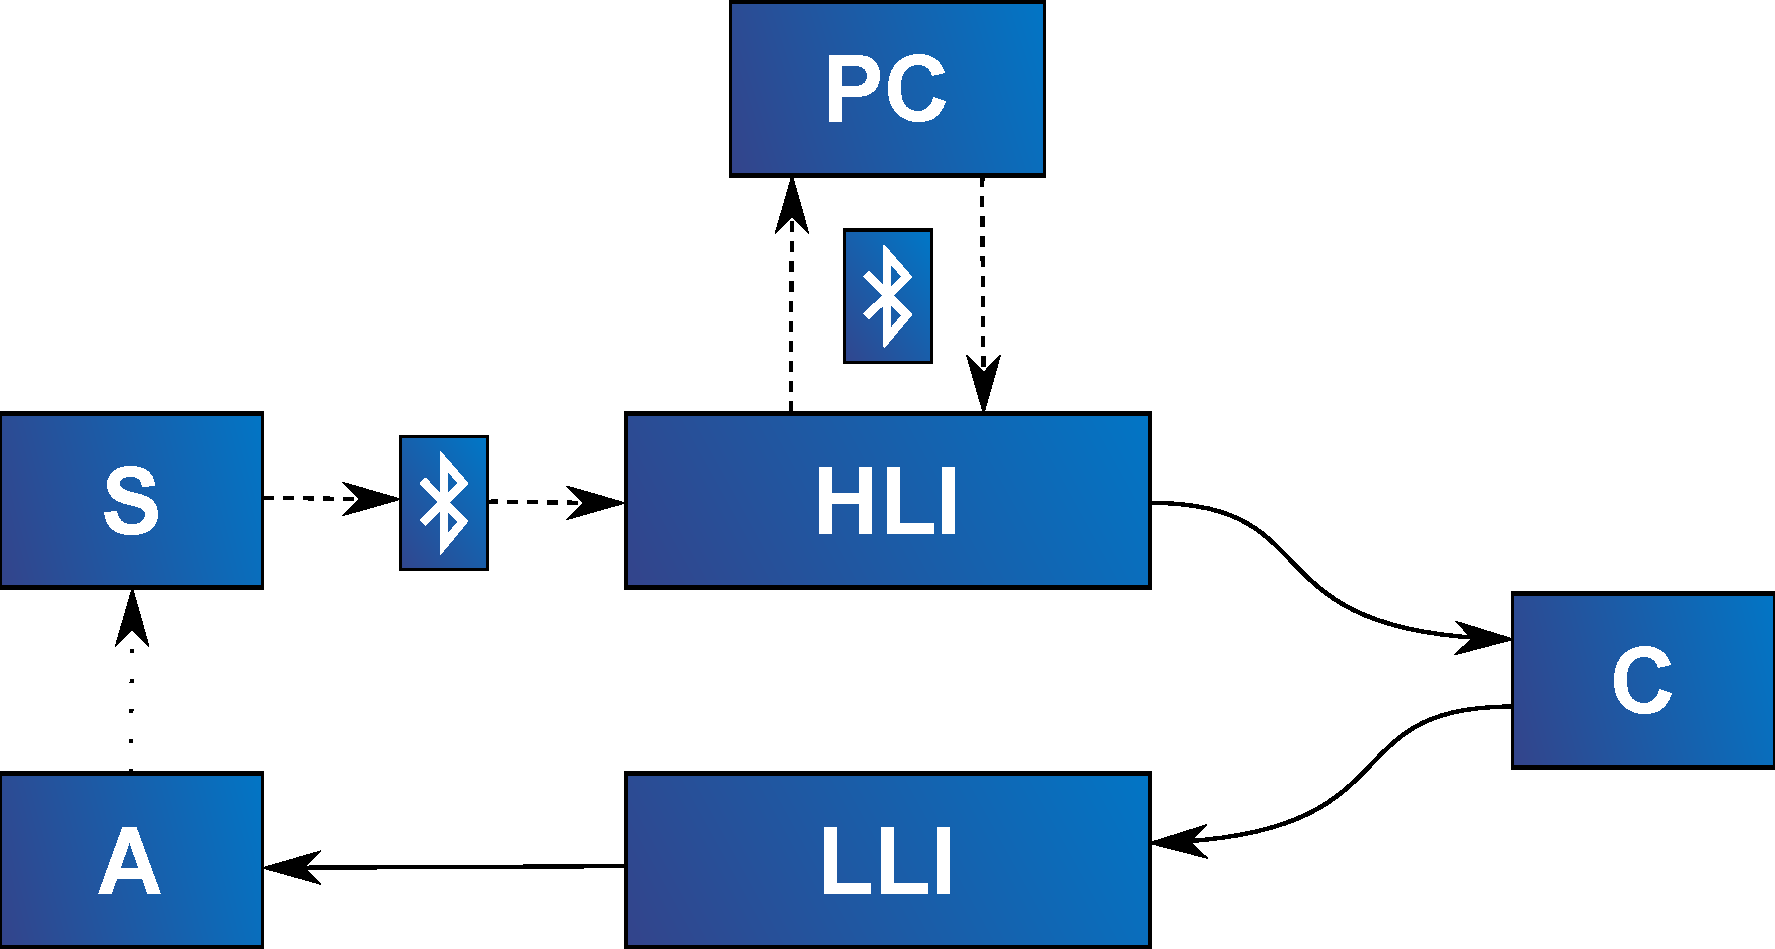
\includegraphics[width=0.8\textwidth]{img2/LogicalLayout}
	\caption{The logical layout of the system}
	\label{fig:LogicalLayout}
\end{figure}

The High Level Interface (HLI) processes the position and orientation sensor data input from Bluetooth serial port. During regular navigation the HLI applies the filtering to the inputs, then outputs the estimated orientation divergence from the path, and the estimated distance from the path. The Controller (C) processes this data and returns the required inputs to the system. The LLI processes this physical signal and transforms them to PWM signals, then applies it to the power electronics and the Actuators (A), which will have the final effect on the system.

It’s important to note in this diagram, that the Controller and is separated from the rest of the software. This enables the user to radically modify the configuration of the robot, or try multiple controller implementations and switch between them real-time. The 
Such a switching system can handle possibly expected failures and breakdowns up to a certain level (like the malfunction of one of the engines of a twin-propeller aircraft).
